\section{Introduction}
\label{sec:introduction}

Nowadays, PC and smartphone running the commodity operating systems, which are
ubiquitous in home, commercial, government and military settings, become
significantly indispensable in our life. According to a report from Gartner
\cite{Gartner}, the worldwide PC shipments totaled 82.6 million units just in
the fourth quarter of 2013. The most popular operating systems on PC are
Windows, Linux and Mac OS. Various applications are installed and executed on
the commodity operating system every day. Besides PC, recent years have also
experienced explosive growth of smartphone sales. Inevitably, the rise in the
popularity of smartphones also makes them an attractive target for attacks.
According to the report from Canalys \cite{Canalys}, the year of 2011 marks as
the first time in history that smartphones have outsold PCs. Their booming
popularity can be partially attributed to their improved functionality and
convenience for end users. 

PCs are used for a variety of daily works such as checking emails, video
conference and data processing. Smartphones are also no longer basic devices
for making phone calls and receiving text messages, but powerful platforms,
with comparable computing and communication capabilities to commodity PCs, for
video conference, gaming, and even online shopping. Generally, different
applications have disparate level of security requirement. For instance, on a
smartphone running Android, the online banking application has a higher level
of security requirement than the Angry Birds.

The execution of mutually mistrusting software brings security trouble to the
commodity operating systems. Suppose the PC is running a Linux operating
system. The user might use the PC to view a lot of PDF files every day. The PDF
file injected with malware is able to infect the operating system because of
the complex interface between the application and the operating system. Latter,
the user may login into the online bank account to check the deposit. As the
underpinning privileged operating system kernel, including keyboard driver, has
already been compromised, the browser's privacy, i.e., the user's credentials,
will be stolen by the attacker.

Another example is on a smartphone running an Android operating system. Users
are suggested to download Android applications from official website, such as
Google Online Store. However, many users download repacked applications, e.g.,
games, from the untrusted third-party website. For instance, without
protection, the malicious repacked game is able to elevate the privilege,
compromise the Android runtime and even the Linux kernel. The compromised
Android operating system is able to infect the privacy and integrity of other
applications, e.g., the user's identification of Facebook.

In this paper, we discuss the solutions for the problems introduced by the
execution of mutually mistrusting software. We formulate the problems into
three sub-problems. The first problem is to protect the secure application or
sensitive PAL (Pieces of Application Logic) from the untrusted operating
system. Commodity operating systems entrusted with securing sensitive data are
remarkably large and complex, and consequently, frequently prone to compromise.
The privacy and integrity of the application are expected to be protected even
in the event of a total OS compromise. Solutions to this problem have a variety
of applications in real life from protecting the privacy and integrity of the
certificate generation process on a CA server to isolating the sensitive list
of Transaction Authentication Numbers (TAN) from the untrusted Android
operating system on a smartphone.

The second problem is to isolate the untrusted application or an untrusted
piece of code from the operating system. Modern commodity operating systems are
underpinning many applications from different sources. The complex interface
between the application and the operating system opens a large attack surface
for the misbehaving application to compromise the rest of the operating system.
The operating system can be compromised by a piece of native code downloaded
and executed by the web browser with mechanisms such as ActiveX and NPAPI, or
an Android application infected by DKFBootKit \cite{DKFBootKit}.

The third problem is how to establish the two-way protection, that is, to
protect the application from the operating system while to protect the
operating system from the application. We rethink the security model and argue
that a two-way sandbox is desired.  We discuss MiniBox \cite{MiniBox}, the
first paper whose objective is to remove the trust between applications and the
operating system on the Platform as a Service (PaaS) cloud computing.

\begin{figure*}[htb]
\centering
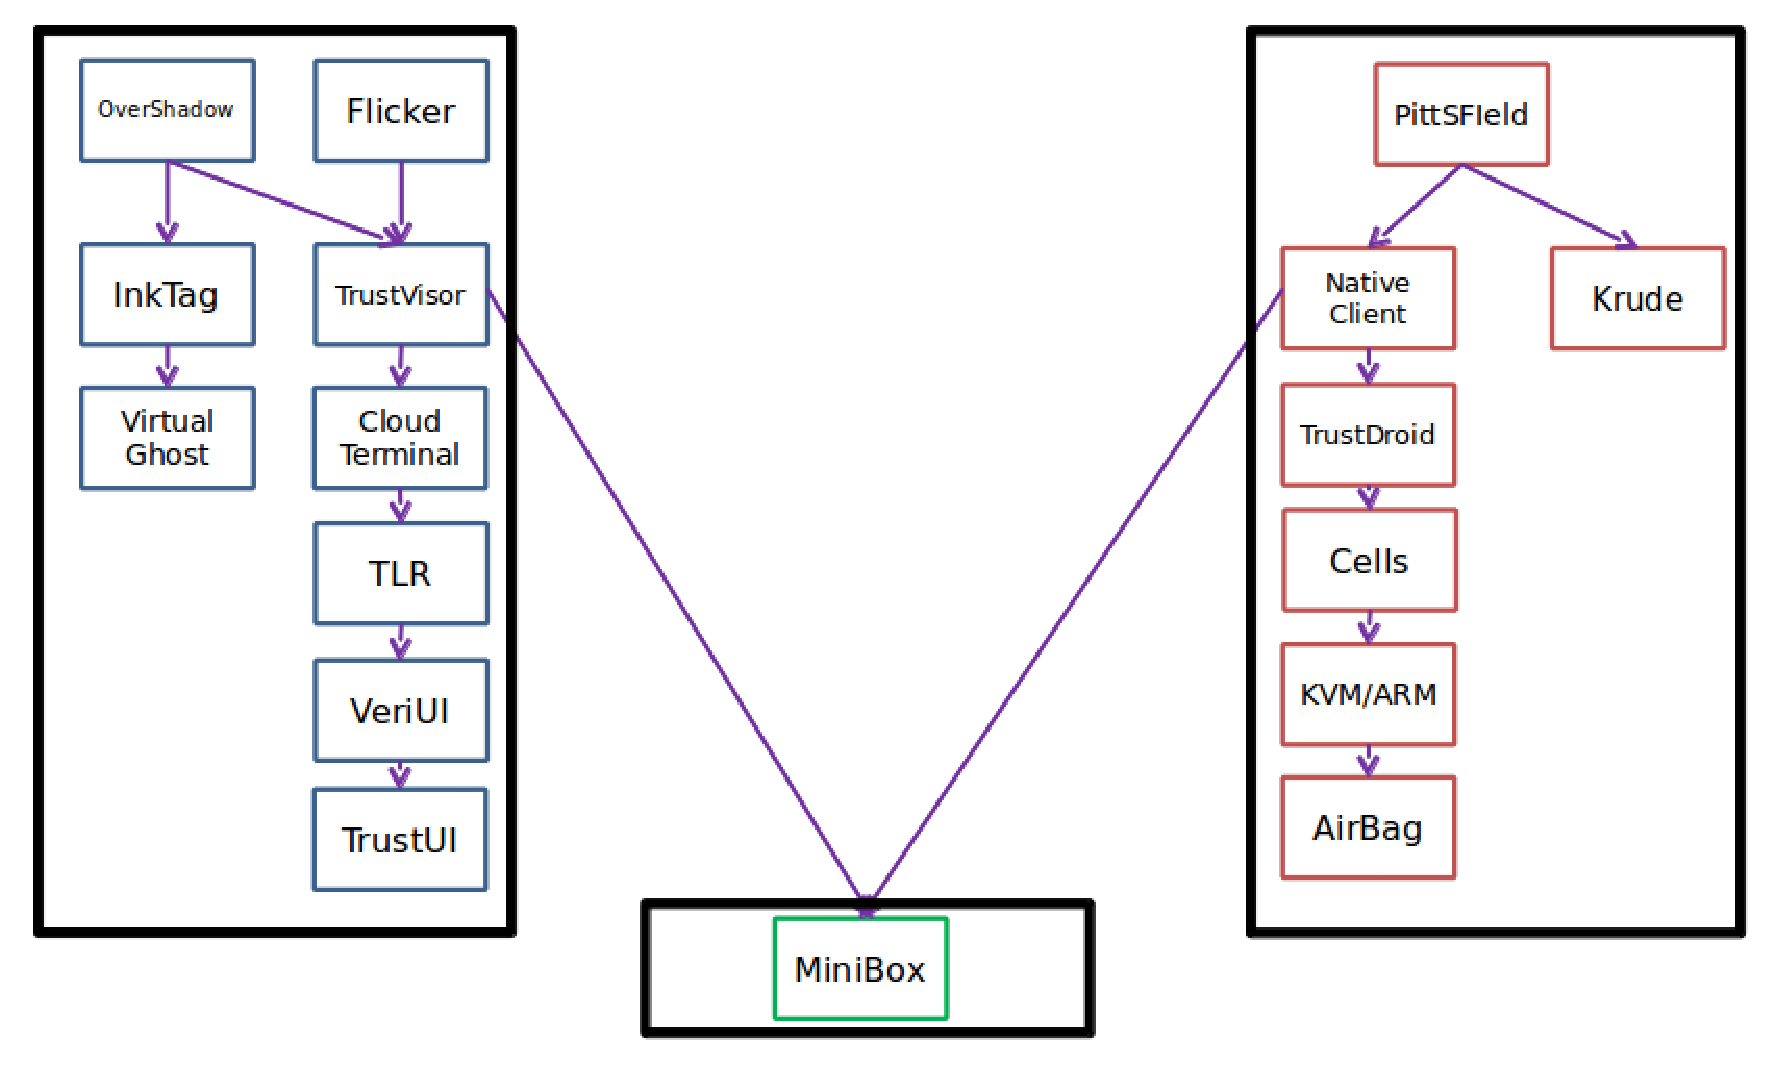
\includegraphics[width=1.5\columnwidth]{figures/evolution.eps}
\caption{Evolution graph of prior works. The left branch includes prior works
when application is trusted but OS is malicious. The right branch includes
prior works when application is untrusted but OS is benign. MiniBox is the
combination of two branches.}
\label{fig:evolution}
\end{figure*}

In this paper, we discuss the evolution of prior works. We organize previous
works based on the problems classification and essential design considerations
when building solutions. The evolution graph of prior works on the three
problems is in Figure \ref{fig:evolution}. In section \ref{sec:problem1}, we
discuss the protection of secure application from the untrusted operating
system. Section \ref{sec:problem2} is about the isolation of untrusted
application from benign operating system. In section \ref{sec:problem3}, we
discuss MiniBox \cite{MiniBox}, the most up-to-date research paper on removing
trust between application and the underpinning operating system. 
